\documentclass[border=10pt]{standalone}
\usepackage{tikz}
\usetikzlibrary{trees,positioning,shadows,shapes}

\begin{document}

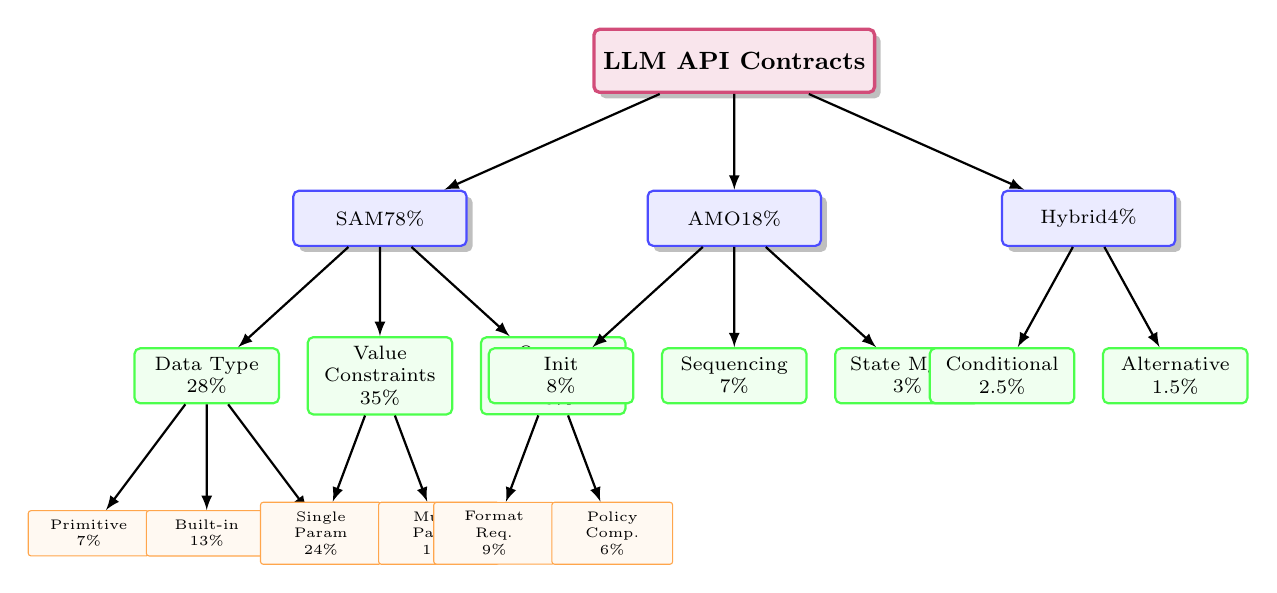
\begin{tikzpicture}[
    level 1/.style={sibling distance=4.5cm, level distance=2cm},
    level 2/.style={sibling distance=2.2cm, level distance=2cm},
    level 3/.style={sibling distance=1.5cm, level distance=2cm},
    main/.style={
        rectangle,
        draw=purple!70,
        fill=purple!10,
        very thick,
        rounded corners=2pt,
        minimum height=0.8cm,
        minimum width=2.5cm,
        font=\small\bfseries,
        drop shadow
    },
    category/.style={
        rectangle,
        draw=blue!70,
        fill=blue!8,
        thick,
        rounded corners=2pt,
        minimum height=0.7cm,
        minimum width=2.2cm,
        font=\scriptsize,
        drop shadow
    },
    subcategory/.style={
        rectangle,
        draw=green!70,
        fill=green!6,
        thick,
        rounded corners=2pt,
        minimum height=0.6cm,
        minimum width=1.8cm,
        font=\scriptsize,
        text width=1.6cm,
        align=center
    },
    subsubcategory/.style={
        rectangle,
        draw=orange!70,
        fill=orange!5,
        thin,
        rounded corners=1pt,
        minimum height=0.5cm,
        minimum width=1.4cm,
        font=\tiny,
        text width=1.3cm,
        align=center
    },
    edge from parent/.style={draw, -latex, thick}
]

% Root
\node[main] {LLM API Contracts}
    % Single API Method (SAM) - 78%
    child {
        node[category] {SAM\\78\%}
        child {
            node[subcategory] {Data Type\\28\%}
            child {node[subsubcategory] {Primitive\\7\%}}
            child {node[subsubcategory] {Built-in\\13\%}}
            child {node[subsubcategory] {Structured\\8\%}}
        }
        child {
            node[subcategory] {Value\\Constraints\\35\%}
            child {node[subsubcategory] {Single\\Param\\24\%}}
            child {node[subsubcategory] {Multi-\\Param\\11\%}}
        }
        child {
            node[subcategory] {Output\\Constraints\\15\%}
            child {node[subsubcategory] {Format\\Req.\\9\%}}
            child {node[subsubcategory] {Policy\\Comp.\\6\%}}
        }
    }
    % API Method Order (AMO) - 18%
    child {
        node[category] {AMO\\18\%}
        child {node[subcategory] {Init\\8\%}}
        child {node[subcategory] {Sequencing\\7\%}}
        child {node[subcategory] {State Mgmt\\3\%}}
    }
    % Hybrid (H) - 4%
    child {
        node[category] {Hybrid\\4\%}
        child {node[subcategory] {Conditional\\2.5\%}}
        child {node[subcategory] {Alternative\\1.5\%}}
    };

\end{tikzpicture}

\end{document}
